\documentclass[a4paper, 11pt]{article}
\usepackage[utf8]{inputenc}
\usepackage[swedish]{babel}
\usepackage{hyperref}
\usepackage[margin=0.5in]{geometry}
\usepackage{graphicx}
\usepackage{amsmath}
\usepackage[arrowdel]{physics}

\newcommand{\integ}[5][]{\int\limits_{#2}^{#3}\dd[#1]{#4}#5}

\title{Sammanfattning av SE1055 Hållfasthetslära}
\author{Yashar Honarmandi \\ yasharh@kth.se}
\date{\today}

\begin{document}

\maketitle

\begin{abstract}
	Denna sammanfattningen innehåller centrala definitioner och satser i SF1672 Flervariabelanalys.
\end{abstract}

\pagenumbering{roman}
\thispagestyle{empty}

\newpage

\tableofcontents

\newpage

\pagenumbering{arabic}

\section{Enaxliga problem}

\paragraph{Krafter på en stång}
Betrakta en stång med tvärsnittsarea $A$ som utsätts för en kraft $P$ i varje ända, med motsatt riktning i varje ända, som visad i figur \ref{fig:cylinder_forces}.
\begin{figure}[!ht]
	\centering
	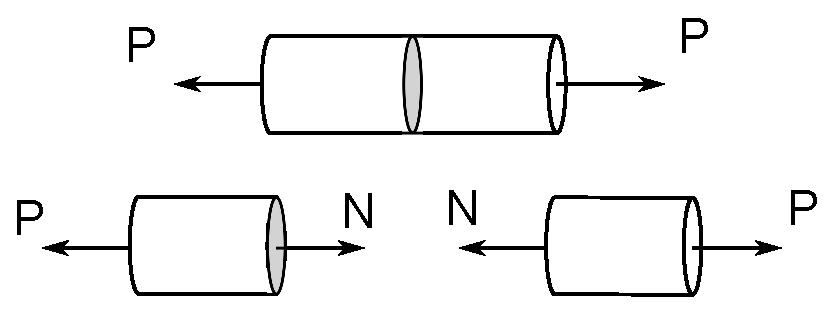
\includegraphics[width = 0.5\textwidth]{./Images/cylinder_forces.eps}
	\caption{Illustration av en stång som utsätts för en dragkraft och de orsakade inre krafterna.}
	\label{fig:cylinder_forces}
\end{figure}

Kraften $P$ i änderna propageras som inre krafter i stången. Om vi betraktar det indikerade tvärsnittet, manifesteras den inre kraften som en normalkraft på varje halva. Om vi definierar positiv riktning för normalkraften och dragkraften som i figuren, ger kraftjämvikten att $N = P$. Om dragkraften blir en tryckkraft, ändrar givetvis normalkraften riktning.

\paragraph{Spänning}
I hållfasthetslära är vi intresserade av påkänningen på materialet. Den beror av beloppet av normalkraften, men kan även spridas ut över tvärsnittet. Därför definierar vi spänningen
\begin{align*}
	\sigma = \frac{N}{A}.
\end{align*}
Jämvikten från innan ger
\begin{align*}
	\sigma = \frac{P}{A}.
\end{align*}

\paragraph{Deformation}
När en stång utsätts för spänning, kommer den att deformeras. Mer specifikt kommer den förlängas med en längd $\delta$. Eftersom förlängningen av varje del kommer från kraftjämvikten mellan normalkraften och dragkraften, kommer förlängningen för en given dragkraft bero av längden. Vi definierar därför töjningen
\begin{align*}
	\varepsilon	= \frac{\delta}{L_{0}}
\end{align*}
där $L_{0}$ är stångens ursprungliga längd.

\paragraph{Typer av samband i hållfasthetslära}
I hållfasthetsläran har vi tre typer av samband:
\begin{itemize}
	\item samband mellan krafter.
	\item samband mellan deformationer.
	\item konstitutiva samband (beskrivar materialbeteende).
\end{itemize}

\paragraph{Hookes lag}
Om man gör dragningsprov på olika material för små deformationer, blir plottet av $\sigma$ mot $\varepsilon$ approximativt linjär. Från detta får vi Hookes lag:
\begin{align*}
	\sigma = E\varepsilon.
\end{align*}
$E$ är elasticitetsmodulen, och beskrivar hur styvt materialet är.

Kombinationen av det vi har tills nu ger
\begin{align*}
	P = \frac{EA}{L}\delta
\end{align*}
för en homogen stång som utsätts för en dragkraft $P$.

Om ett material komprimeras, visar det sig att det elastiska beteendet ofta är likt, med samma elasticitetsmodul.

\paragraph{Normalspänning}
Vi utvidgar våran definition av spänning till spänningar som fördelas inhomogent över tvärsnittet vid att betrakta en inre kraft $\Delta F$ som verkar på ett arealement $\Delta A$, med riktningar som tidigare. Då definieras normalspänningen som
\begin{align*}
	\sigma = \lim\limits_{\Delta A\to 0}\frac{\Delta F}{\Delta A}.
\end{align*}

\paragraph{Normaltöjning}
Vi utvidgar även definitionen av töjning till töjningar som fördelas ojämnt över stavens längd. Om deformationen i en punkt är $u(x)$, ges töjningen av ett litet element med längd $\Delta x$ av
\begin{align*}
	\varepsilon = \lim\limits_{\Delta x\to 0}\frac{u(x + \Delta x) - u(x)}{\Delta x} = \dv{u}{x}.
\end{align*}
Vi ser av detta att töjningen är linjär, så vi kan addera bidrag till den.

\paragraph{Termoelasticitet}
Låt $T$ beteckna en stångs temperatur. En temperaturändring orsakar en termisk töjning
\begin{align*}
	\varepsilon_{T} = \alpha\Delta T,
\end{align*}
där $\alpha$ är längdutvidgningskoefficienten. Man behöver givetvis utgå från en referenstemperatur.

\paragraph{Allmänt enaxligt tillstånd}
Från det vi har sett hittils, kan vi skriva upp en differentialekvation som beskriver det enaxliga tillståndet.

Betrakta en stång med variabel tvärsnittsyta där det överallt i kroppen verkar en volymskraft $K(x)$ (kraft per volym), samt krafter $P_{\text{V}}$ respektiva $P_{\text{H}}$ i varje ända. Vi betraktar ett litet element med tjocklek $\dd{x}$. I ena ändan verkar kraften $K(x)A\dd{x}$ och en normalkraft $N(x)$ på grund av krafterna på volymelementet till vänster, och i andra ändan verkar en normalkraft $N(x + \dd{x})$ på grund av krafterna på volyemelementet till höger.

Kraftjämvikten ger
\begin{align*}
	N(x + \dd{x}) - N(x) + K(x)A\dd{x} &= 0, \\
	\dd{N}{x} + K(x)                   &= 0.
\end{align*}
Vi inför nu definitionen av töjninc och skriver den som en linjärkombination av bidrag från spänning och termoelasticitet, vilket ger
\begin{align*}
	\varepsilon = \frac{\sigma}{E} + \alpha\Delta T, \\
	\sigma = E(\varepsilon - \alpha\Delta T).
\end{align*}
Kombinerad med definitionen av töjning ger det
\begin{align*}
	\dv{x} (\sigma A) + K(x)A &= 0, \\
	\dv{x} (EA(\varepsilon - \alpha\Delta T)) + K(x)A &= 0, \\
	\dv{x}\left(EA\dv{u}{x}\right) + K(x)A &= \dv{x}(EA\alpha\Delta T).
\end{align*}
Detta kommer med randvillkor, och är typiskt randvillkor i deformationen eller i spänningen. Eftersom spänningen är proportionell mot derivatan av deformationen, motsvarar dessa Dirichlet- respektiva Neumannvillkor.

\section{Koncept i tre dimensioner}

\paragraph{Tvärkontraktion}
När man gör ett dragningsprov på en stång, genomgår den deformation i längdriktning samtidigt som tjockleken minskar. Detta kallas tvärkontraktion. Töjningen $\varepsilon_{t}$ av tjockleken är relaterad till töjningen i längdriktning genom
\begin{align*}
	\varepsilon_{t} = -\nu\varepsilon,
\end{align*}
där $\nu$ är Poissons konstant. Termodynamiken ger att $-1\leq\nu\leq 0.5$.

\paragraph{Skjuvspänning}
Betrakta två plattor som ligger på varandra och dras åt motsatta håll av en kraft $F$ på varje. Om de inte dras isär, balanseras dragkrafterna av krafter i kontaktytan. Låt $A$ vara kontaktytan mellan plattorna. Då definieras skjuvspänningen som
\begin{align*}
	\tau = \frac{F}{A}.
\end{align*}

\paragraph{Deformation från skjuvkrafter}
Betrakta ett rätblock med basarea $A$ och höjd $H$ som dras av motsatt riktade krafter med belopp $F$ på varje sida, illustrerad i figur \ref{fig:rectangle_twist}.
\begin{figure}[!ht]
	\centering
	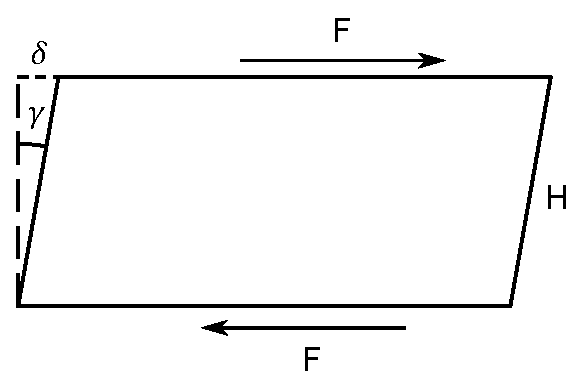
\includegraphics[width = 0.5\textwidth]{./Images/rectangle_twist.eps}
	\label{fig:rectangle_twist}
\end{figure}

Vi kan här definiera skjuvspänningen som
\begin{align*}
	\tau = \frac{F}{A},
\end{align*}
då vi kan tänka oss att plattorna som dras isär är tunna skikt i materialet. Skjuvkrafterna kommer skapa en deformation $\delta$ på en sida motsvarande vridning med en vinkel $\gamma$. Denna vinkeln uppfyller
\begin{align*}
	\tan{\gamma} = \frac{\delta}{H}.
\end{align*}
För små deformationer kan vi approximera
\begin{align*}
	\gamma = \frac{\delta}{H}.
\end{align*}
Experimentellt har man sett att
\begin{align*}
	\tau = G\gamma,
\end{align*}
där $G$ är skjuvmodulen.

\paragraph{Samband mellan materialstorheter}
För ett isotropt material gäller att
\begin{align*}
	G = \frac{E}{2(1 + \nu)}.
\end{align*}

\paragraph{Statiskt bestämta och obestämta problem}
Ett problemt är statiskt bestämt om alla inre krafter och reaktionskrafter kan bestämmas enbart med jämvikt. Detta är möjligt om det verkar maximalt $3$ krafter i planet eller $6$ i rymden.

Om ett problem ej är statiskt bestämt, är det statiskt obestämt. Då räcker icke jämviktsekvationerna, och det motsvarar att man kan ta bort ett element och vara kvar i jämvikt.

\paragraph{Elastisk vridning}
Antag att man har en stång med cirkulärt tvärsnitt fäst i ena ändan som man vrider med ett moment $M_{\text{v}}$ (i varje ända). Detta ger en vinkeldeformation $\theta$ i det yttersta tvärsnittet och $\gamma$ relativt linjen parallellt med stångens riktning. Om stången har en längd $l$ och en radius $a$, ger detta
\begin{align*}
	L\gamma = a\theta.
\end{align*}
Kombinerad med resultatet från delen om skjuvspänning ger detta
\begin{align*}
	\frac{\theta}{L} = \frac{\tau}{G}.
\end{align*}
Antag nu att $\tau = \frac{M_{\text{v}}}{K}$. Detta ger
\begin{align*}
	\frac{\theta}{L} = \frac{M_{\text{v}}}{GK}.
\end{align*}
$K$ är en konstant som beror av stångens geometri.

Hur beräknar vi $K$? Jo, man integrerar momentets differential över tvärsnittet. Vi vet att detta differentialet ges av kraft gånger arm, och det är så skjuvspänningen kommer in.

\paragraph{Balkböjning}
För att beskriva balkar behöver vi införa fler olika sorters inre krafter och moment. Dessa illustreras i figur \ref{fig:beam_forces}.
\begin{figure}[!ht]
	\centering
	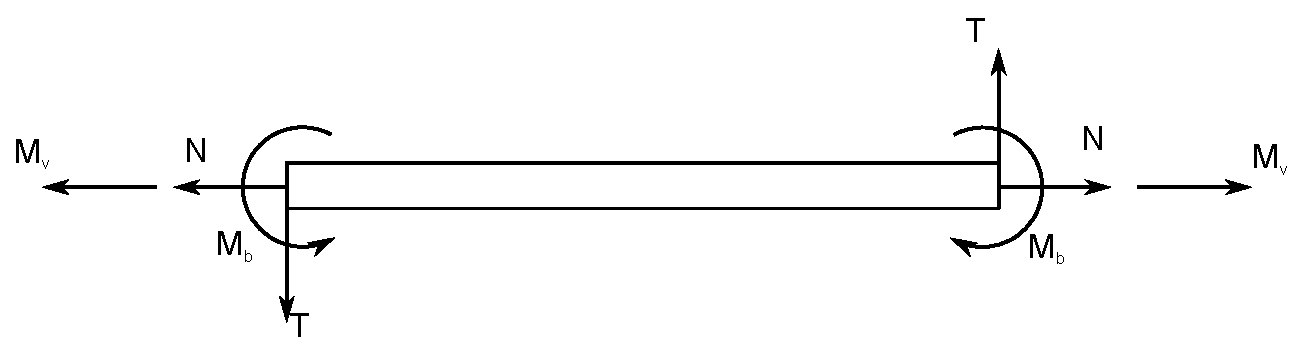
\includegraphics[width = 0.5\textwidth]{./Images/beam_forces.eps}
	\caption{Illustration av inre krafter och moment i en balk.}
	\label{fig:beam_forces}
\end{figure}
Vi har infört normalkraften $N$, tvärkraften $T$, det böjande momentet $M_{\text{b}}$ och det vridande momentet $M_{\text{v}}$.

Låt $u$ vara balkens deformation normalt på dens utsträkning. Vi har från enaxliga tillståndet att
\begin{align*}
	\frac{\Delta u}{L} = \frac{N}{EA}.
\end{align*}
Låt $\theta$ och $\phi$ vara vinklarna för böjning och vridning. Vi har då
\begin{align*}
	\frac{\Delta\theta}{L} = \frac{M_{\text{v}}}{GK},
	\frac{\Delta\phi}{L} = \frac{M_{\text{b}}}{EI}.
\end{align*}

\paragraph{Allmänt tillstånd för en balk}
Snitta nu ut ett element med längd $\dd{x}$ från en balk. Om balken påverkas av en last $q$ per längdenhet, ger kraftjämvikten
\begin{align*}
	T(x + \dd{x}) - T(x) + q(x)\dd{x} = 0,
\end{align*}
vilket ger
\begin{align*}
	\dd{T}{x} = -q.
\end{align*}
Momentjämvikt kring centrum ger
\begin{align*}
	M(x + \dd{x}) - M(x) - (T(x) + T(x + \dd{x}))\dd{x} = 0.
\end{align*}
Bidraget från tvärkraften ges av
\begin{align*}
	T(x) + T(x + \dd{x}) &= 2T(x) + \dv{T}{x}\dd{x} \\
	                     &= 2T(x) - q(x)\dd{x}.
\end{align*}
Insatt i momentjämvikten fås
\begin{align*}
	M(x + \dd{x}) - M(x) - \frac{1}{2}\dd{x}(T(x) + T(x + \dd{x})) = M(x + \dd{x}) - M(x) - T(x)\dd{x} + \frac{1}{2}\dd{x}q(x)\dd{x}.
\end{align*}
Vi försummar nu alla andra ordningens termer, vilket ger
\begin{align*}
	\dv{M}{x} = T.
\end{align*}
Kombinerat med det förra resultatet fås
\begin{align*}
	\dv[2]{M}{x} = -q.
\end{align*}

\paragraph{Randvillkor för balkar}
En balk kan i en given ända vara
\begin{itemize}
	\item fri, vilket ger $T = 0$ och $M = 0$.
	\item fritt upplagd, vilket ger $M = 0$.
	\item glidinspänd, vilket ger $T = 0$.
	\item fast inspönd, vilket ej ger villkor för de inre krafterna och momenterna.
\end{itemize}

\section{Materialers beteende}

\paragraph{Idealplastisk deformation}
De flesta material beter sig så att när de deformeras förbi en viss punkt, deformeras de plastiskt i stället för elastiskt. En approximation för att beskriva detta beteendet är att låta deformationen vara elastisk upp till en töjningsgräns $\varepsilon_{\text{s}}$, och låta $\sigma$ vara konstant lika med en sträckgräns $\sigma_{\text{s}}$ för större töjningar.

När lasten sedan tas bort, kommer stången förkortas igen tills lasten blir lika med noll. Denna kontraktionen är parallell med det elastiska regimet, och konsekvensen är att man får en permanent deformation.

\paragraph{Enkelriktad fiberkomposit}
En enkelriktad fiberkomposit är ett material som består av fibrar som alla är parallella och ett omkransande material som kallas en matris. Matrisen och fibern finns i volymfraktioner $v_{\text{m}}$ respektiva $v_{\text{f}}$, och de har elasticitetsmoduler $E_{\text{m}}$ respektiva $E_{\text{f}}$.

Som en modell för belastning längsmed fibrernas riktning betraktar vi uppställningen som ges i figur \ref{fig:fiber_composite_parallel}.
\begin{figure}[!ht]
	\centering
	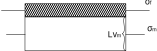
\includegraphics[width = 0.5\textwidth]{./Images/fiber_composite_parallel.eps}
	\caption{Illustration av en del av en enkelriktad fiberkomposit som belastas längsmed fiberns riktning.}
	\label{fig:fiber_composite_parallel}
\end{figure}

Kraftjämvikten ger $F = \sigma A$. Vi antar att den utskurna biten är ett rätblock, så de två delarna har tvärsnittsareor som ges av totala tvärsnittsarean och volymfraktionerna. Detta ger
\begin{align*}
	F = \sigma A = (\sigma_{\text{f}}v_{\text{f}} + \sigma_{\text{m}}v_{\text{m}})A.
\end{align*}
Därmed ges spänningen av
\begin{align*}
	\sigma = \sigma_{\text{f}}v_{\text{f}} + \sigma_{\text{m}}v_{\text{m}}.
\end{align*}
Vi antar att fibern och matrisen inte glider relativt varandra, och därmed har de samma deformation och töjning. Hookes lag ger
\begin{align*}
	\sigma_{\text{f}} = E_{\text{f}}\varepsilon, \sigma_{\text{m}} = E_{\text{m}}\varepsilon,
\end{align*}
vilket insatt i uttrycket ovan ger
\begin{align*}
	\sigma &= v_{\text{f}}E_{\text{f}}\varepsilon + v_{\text{m}}E_{\text{m}}\varepsilon \\
	       &= (v_{\text{f}}E_{\text{f}} + v_{\text{m}}E_{\text{m}})\varepsilon.
\end{align*}
För hela biten med fiberkomposit ger Hookes lag då
\begin{align*}
	E_{\text{L}} = v_{\text{f}}E_{\text{f}} + v_{\text{m}}E_{\text{m}}
\end{align*}
som elasticitetsmodulen vid längsgående spänning. Vi får även
\begin{align*}
	\sigma_{\text{f}} &= E_{\text{f}}\varepsilon \\
	                  &= \frac{E_{\text{f}}}{E_{\text{L}}}\sigma
\end{align*}
som spänning i fibrerna, och motsvarande för matrisen.

På samma sättet beskriver vi även fallet när spänningen går på tvärs av fibrernas riktning, som illustrerad i figur \ref{fig:fiber_composite_normal}.
\begin{figure}[!ht]
	\centering
	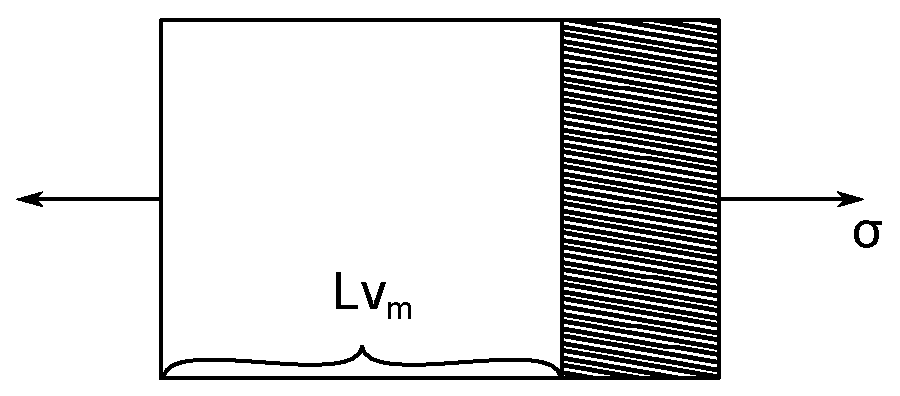
\includegraphics[width = 0.5\textwidth]{./Images/fiber_composite_normal.eps}
	\caption{Illustration av en del av en enkelriktad fiberkomposit som belastas normalt på fiberns riktning.}
	\label{fig:fiber_composite_normal}
\end{figure}

Här kan vi snitta och se att $\sigma_{\text{f}} = \sigma_{\text{m}}$. Den totala förlängningen i denna biten ges av
\begin{align*}
	\delta = \delta_{\text{f}} + \delta_{\text{m}} = L_{\text{f}}\varepsilon_{\text{f}} + L_{\text{m}}\varepsilon_{\text{m}}.
\end{align*}
Töjningen ges då av
\begin{align*}
	\varepsilon &= \frac{\delta}{L_{\text{f}} + L_{\text{m}}} \\
	            &= \varepsilon_{\text{f}}\frac{L_{\text{f}}}{L_{\text{f}} + L_{\text{m}}} + \varepsilon_{\text{m}}\frac{L_{\text{m}}}{L_{\text{f}} + L_{\text{m}}} \\
	            &= v_{\text{f}}\varepsilon_{\text{f}} + v_{\text{m}}\varepsilon_{\text{m}}.
\end{align*}
Hookes lag ger
\begin{align*}
	\varepsilon &= v_{\text{f}}\frac{\sigma}{E_{\text{f}}} + v_{\text{m}}\frac{\sigma}{E_{\text{m}}},
\end{align*}
och vi ser att
\begin{align*}
	\frac{1}{E_{T}} = \frac{v_{\text{f}}}{E_{\text{f}}} + \frac{v_{\text{m}}}{E_{\text{m}}}.
\end{align*}

\paragraph{Ideallastisk vridning}
Vi inför idealplastiska material även i vridningssammanhang. Dessa beter sig analogt till idealplastiska material under dragning, där vi ersätter töjningen med skjuvvinkeln $\gamma$, spänningen med skjuvspänningen $\tau$, töjningsgränsen med en vinkelgräns $\gamma_{\text{s}}$ och sträckgränsen med en skjuvgräns $\tau_{\text{s}}$.

\paragraph{Knäckning}
Om man t.ex. belastar en balk i dens längdriktning med en last som är större än en viss kritisk last, kommer balken snabbt böjas och nå ett nytt jämviktsläge. Detta kommer av att ursprungsläget är en instabil jämviktspunkt, så den minsta störning kommer att få den att anta ett stabilt jämviktstillstånd. Detta är ett exempel på ett instabilitetsfenomen.

\paragraph{Plasiticitetsteori i tre dimensioner}
I tre dimensioner inför vi effektivspänningen $\sigma_{\text{e}}$, som beror av spänningsmatrisen, och kräver $\sigma_{\text{e}}(S) = \sigma_{\text{s}}$ för att plasticitet skall inträda. Vi kommer undersöka detta för isotropa material.

Vi kan välja huvudspänningsriktningarna som koordinatsystem. Då kan effektivspänningen reduceras till $\sigma_{\text{e}}(S) = \sigma_{\text{e}}(\sigma_{1}, \sigma_{2}, \sigma_{3})$. Plasticitetskriteriet definierar då en yta i tre dimensioner. Av rimlighetsskäl kan ytan inte skära origo.

Vi kan kräva vissa saker av flytvillkoret, till exempel
\begin{itemize}
	\item det skall vara oberoende av eventuellt hydrostatiskt tryck, dvs. $\sigma_{\text{e}}(\sigma_{1}, \sigma_{2}, \sigma_{3}) = \sigma_{\text{e}}(\sigma_{1} - p, \sigma_{2}- p, \sigma_{3}- p) = \sigma_{\text{s}}$. Detta implicerar att ytan som definieras av flytvillkoret är en cylinderyta med riktning $(1, 1, 1)$.
	\item det uppfyller ett enaxligt flytvillkor, dvs. att om någon huvudspänning är $\sigma_{\text{s}}$ och de andra är $0$, uppfylls flytvillkoret.
	\item det är oberoende av reversering av spänningstillståndet, dvs. om alla huvudspänningar byter tecken är flytvillkoret uppfyld.
	\item det är isotropiskt, dvs. permutation av huvudspänningarna ger fortfarande att flytvillkoret är uppfyld.
\end{itemize}
Från detta kan vi dra slutsatsen att vi endast behöver titta på en $30\degree$ sektor av ytan, då symmetrier ger resten av ytan.

\paragraph{von Mises}
von Mises lösning är att säja att denna sektorn är en cirkelbåge. Det finns en formel för denna.

\paragraph{Tresca}
Trescas lösning är att säja att denna sektorn är en rät linje. Det finns en formel för denna.

\paragraph{Jämförelse}
Om man jämför Trescas och von Mises teorir, blir det störst skillnad vid ren vridning. Trescas villkor är en mer konservativ gräns än von Mises, då den allmänt ligger närmare origo. Trescas villkor har hörn, och är därför svår numeriskt. Båda funkar ändå rätt bra när man jämför med experiment.

\paragraph{Utmattning}
Utmattning är fenomenet som uppstår när brott uppstår under spänningsgränser. Det som händer är att spänningsgränsen blir lägre i materialet av cyklisk deformation, och att den tenderer mot en utmattningsgräns.

För att beskriva cykliska belastningar, inför vi begreppen minimumspänning, maximumspänning, amplitudspänning, mittspänning och spänningsförhållande. Vi har
\begin{align*}
	\sigma_{\text{a}} &= \frac{\sigma_{\text{max}} - \sigma_{\text{min}}}{2}, \\
	\sigma_{\text{m}} &= \frac{\sigma_{\text{max}} + \sigma_{\text{min}}}{2}, \\
	R                 &= \frac{\sigma_{\text{min}}}{\sigma_{\text{max}}}.
\end{align*}

\paragraph{Dragprovning och S-N-diagram}
För att testa materialers utmattningsegenskaper, kan man utsätta ett prov för varierande spänningar. Det vanlige är rent varierande eller pulserande spänningar. För en given spänningsamplitud kan man mäta hur många cykler provet kan gå igenom innan brott, och detta kan plottas i ett S-N-diagram. I ett sånt diagram kan man också rita olika kurvor för olika brottsannolikheter.

Av detta kan man läsa av brottgränsen $\sigma_{\text{B}}$ vid låga $N$ och utmattningsgränsen $\sigma_{\text{u}}$ vig höga $N$. Om man belastar provet med en spänning som är lägre än detta, har provet oändlig livslängd. Kurvan har typiskt en omvänd sigmoid form, och gränslivslängden $N{\text{g}}$ definieras som det $N$ där kurvan igen blir platt. Om spänningen är pulserande, betacknas utmattningsgränsen som $\sigma_{\text{up}}$. Motsvarande gränser kan även införas vid böjning eller böjning med rotation.

\paragraph{Haigh-diagram}
Ett Haigh-diagram är en representation av alla kombinationer av mittspänning och amplitudspänning som ger brott. Vi kommer dock förhålla oss till förenklade Haigh-diagram. Dessa konstrueras vid att dra räta linjer mellan olika punkter.

Den första punkten är $\sigma_{\text{m}} = 0, \sigma_{\text{a}} = \sigma_{\text{u}}$, som motsvarar rent växlande belastning. Den andra punkten är en rent växlande spänning $\sigma_{\text{a}} = \sigma_{\text{m}} = \sigma_{\text{up}}$. Den tredje punkten fås från ett rent statiskt dragprov $\sigma_{\text{a}} = 0, \sigma_{\text{m}} = \sigma_{\text{B}}$. Linjerna mellan dessa är ett Haigh-diagram. Man kan även förfina vid att lägga till en linje mellan $\sigma_{\text{s}}$ på båda axlarna för att ta höjd för plasticering. Då blir Haigh-diagrammet den kurvan som ligger lägst i diagrammet.

För att undersöka om den givna lasten ger brott, ritar man punkten in i Haigh-diagrammet. Om punkten är under kurvan, sker inte brott.

\paragraph{Dimensionering}
I vanliga fall vill man inte göra val baserad på gränserna utan med lite marginaler. Då kan man välja efter gränserna, fast multiplicerad med en faktor
\begin{align*}
	1 - \frac{\lambda}{K_{\text{f}}K_{\text{r}}K_{\text{d}}}.
\end{align*}
De olika faktorerna här förtjäner lite förklaring.

$\lambda$ är en faktor som tillkommer på grund av materialkvalitet. I moderna material är denna endast viktig för gjutna komponenter.

$K_{\text{f}}$ beror igen av en geometrisk faktor $K_{\text{t}}$. Tack, hållf. Om det finns variationer i komponentens tvärsnitt längsmed dens längd, beräknar man nominell spänning med hjälp av den minsta tvärsnittsdatan för att uppskatta den största spänningen som förekommer. Den maximala spänningen i komponenten är dock större än detta, tydligen, och kvoten mellan den maximala och nominella spänningen är $K_{\text{t}}$. $K_{\text{f}}$ fås med hjälp av sambandet $K_{\text{f}} = 1 + q(K_{\text{t}} - 1)$, där $q$ är en materialberoende storhet.

$K_{\text{r}}$ beskriver ytfinheten, som visar sig påverka hållfastheten. Denna beror igen av medelytavvikelsen $R_{\text{a}}$.

$K_{\text{d}}$ beror av provets storlek. Storleken spelar in på ett sätt som inte är helt klart.

När man nu har konstruerat sitt förbättrade Haigh-diagram, kan man bestämma säkerhetsfaktorer med hjälp av avstånd i Haigh-diagrammet. Hur detta görs beror på vilken sorts last man har, och beskrivs (förhoppningsvis) i formelbladet.

\end{document}
